\documentclass[conference,10pt]{IEEEtran}
\usepackage{flushend}
\usepackage{lastpage}
\usepackage[utf8]{inputenc}
\usepackage{mathptmx}
\usepackage[dvipsnames]{xcolor}
\usepackage[T1]{fontenc}
\usepackage[english]{babel}
\usepackage{array}
\usepackage{url}
\usepackage{hyperref}
\usepackage[caption=false]{subfig}
\usepackage{microtype}
\usepackage{graphicx}
\usepackage[binary-units,per-mode=symbol]{siunitx}
\usepackage{cite}
\usepackage{multicol}
\usepackage{graphicx}
\usepackage{subfigure}

\def\UrlBreaks{\do\/\do-}

\hypersetup{
  colorlinks=true,% Color URLs with urlcolor
  linkcolor=black,% The color for internal (cross-reference) links
  urlcolor=blue,% The color for URLs (hyperlinks)
  citecolor=black,
  pdftitle={Internet Usage during COVID-19 in the US}
}

\urlstyle{same}

% TODO
% - http://www.oecd.org/coronavirus/policy-responses/keeping-the-internet-up-and-running-in-times-of-crisis-4017c4c9/


\begin{document}
\title{Internet Usage during COVID-19 in the US}

\author{
    \IEEEauthorblockN{Jessica Moreira}
    \IEEEauthorblockA{
        Barnard College\\
        New York, NY 10027\\
        Email: jdm2240@barnard.edu
    }
    \and
    \IEEEauthorblockN{Jan Janak, Henning Schulzrinne}
    \IEEEauthorblockA{
        Dept. of Computer Science\\
        Columbia University\\
        New York, NY 10027\\
        Email: \{janakj,hgs\}@cs.columbia.edu
    }
}

\maketitle

\begin{abstract}
The COVID-19 outbreak has changed the way that people interact. With the new stay-at-home and social distancing orders, most activities that people were used to changed drastically, e.g., going to work and classes, living on campuses and traveling. In this new social environment, since early March people in the US were required to quarantine and do all their activities from home. Thus, in this project we researched how COVID-19 impacted Internet usage in the US. While analyzing the fixed broadband raw data sets collected by the Federal Communications Commission (FCC), we were able to identify how aspects of Internet usage such as amounts of data downloaded and uploaded by users and the average download and upload speed changed due to COVID-19. Moreover, through this analysis, we could also learn about how people have changed their behaviors while using Internet during COVID-19.
\end{abstract}

\section{Introduction}
\label{sec:introduction}

In early March, the US was hit by the COVID-19 outbreak. In order to control the spread of the virus and flatten the infection curve, states throughout the country implemented stay-at-home orders which forced people to quarantine. Thus, as people started quarantining at home, many started executing their daily activities, e.g., having social gatherings from home in an online environment.

Thus, considering this new format of social interaction caused by COVID-19, this study aims to understand how this virus has impacted Internet usage in the United States. It identifies the changes in Internet usage caused by the COVID-19 outbreak, e.g., change in the average downloaded and uploaded data consumption, in the average download and upload speed, in the peak periods of usage, and in latency. By observing the changes in the way that Internet has been used, this study also infers and presents information about people's behavior during COVID-19, e.g., if people complied with stay at home orders, engaged in online learning, and worked from home.

In the following sections of the paper we present related work about the impacts of COVID-19 in Internet usage (Section \ref{sec:related-work}), information about the data set (Section \ref{sec:datasets}) and the environment used to process and analyze the data (Section \ref{sec:methodology}) and then the results achieved by analyzing the data (Section \ref{sec:data-analysis}). Moreover, we also present the challenges that we faced while executing this project (Section \ref{sec:challenges}). Finally, we conclude and discuss future work in Section \ref{sec:conclusion}.

\section{Related Work}
\label{sec:related-work}

A small number of studies have been published while we were working on analyzing FCC MBA data. Feldmann et al. examined the effects of lockdowns on residential Internet traffic using data obtained from a European ISP and Internet Exchange Points (IXP) in Europe and the US East Coast\cite{feldmann2020lockdown}. They found that residential traffic increased by 15-20 \% within a week. Campus network traffic volume decreased, except for the traffic generated by remote working and learning applications. Overall, Internet infrastructure was able to handle the increase.

\nocite{openvault}
\nocite{uk-home-broadband-performance}
\nocite{samknows-cdn}
\nocite{samknows-video-streaming}
\nocite{samknows-video-conferencing}
\nocite{lutu2020characterization}
\nocite{liu2020characterizing}
\nocite{partridge2003internet}

According to the study about Internet performance conducted by Kovacs, after the staying-home orders started in European countries and in the US, the American broadband network has performed well compared to the European one. The numbers show that traffic of data in the US grew up to \SI{30}{\percent} in a month and that even with this increase, the average download speed in the US was \SI{138}{\mega\bit\per\second}. On the other hand, the EU showed a mean download speed of \SI{75}{\mega\bit\per\second}, showing that the average download speed in the US was \SI{83}{\percent} higher than in the EU after the COVID-19 outbreak. Kovacs also argues that the US has had a better broadband network performance than the EU due to its diversified kinds of technology, which made the country not dependent on DSL. Only \SI{18}{\percent} of the US broadband Internet uses DSL while in the EU this number is approximately \SI{50}{\percent} \cite{kovacs}.

Moreover, the article \textit{Stealth CEO: Asymmetric broadband speeds cause strain during work from home efforts} \cite{robuck} points out that people who are currently working from home have faced some challenges to open all their work applications and have been using more cloud services. According to Robuck, Internet traffic caused by these cloud services increased \SI{32}{\percent} since staying-home orders started in the country. Moreover, it has been confirmed that people have experienced an asymmetrical connection which has directly slowed the upstream speed.

In addition to that, according to the article \textit{COVID-19: How Cable's Internet Networks Are Performing} \cite{ncta}, since March 1st, the downstream peak in the US increased by \SI{8.4}{\percent} while the upstream peak increased by \SI{23.1}{\percent}. In addition to that, the conducted study showed that the upstream peak hours shifted from evenings to afternoons and that a more local analysis showed that in New York state these numbers increased by \SI{9}{\percent} and \SI{23.4}{\percent} respectively.

Finally, according to Frankel \cite{frankel}, the average down streams in urban spaces in March 16th was \SI{5.1}{\giga\byte} - more than double of the down streams value registered nine weeks before. In addition to that, Frankel affirms that according to Nilsen, video streaming consumption increased \SI{61}{\percent} in the US since early March.

\section{Datasets}
\label{sec:datasets}

% TODO: Add subsection about privacy and ethical considerations, discussing how our analyses fit into these.

The Federal Communications Commission (FCC) runs a program called Measuring Broadband America (MBA) which measures the broadband Internet usage and performance in the US \cite{mba}. The FCC selected around 4,000 to 5,000 volunteers with a broadband Internet connection. Each volunteer receives a Whitebox, a dedicated device provided by SamKnows in order to measure the performance of their broadband Internet connection \cite{sam}. The Whitebox performs active and passive measurements and generates data that is collected by the FCC. All deployed Whiteboxes generate approximately \SI{20}{\giga\byte} of data per month. The FCC makes the collected data publicly available on their website \cite{data}.

Since 2011, the FCC has been publishing annual reports that summarize the state of the US broadband performance. The reports are based on the collected data and additional information collected and cross-validated from the selected broadband Internet Service Providers (ISPs) from four different regions of the country. This information included in the reports represents approximately \SI{80}{\percent} of the total US population \cite{mba-studies}.

For this study, we focused on using the collected MBA (raw) data to analyze the changes in Internet usage caused by COVID-19. We worked with the data collected from January 2019 to March 2020. By analyzing these data sets, we were aiming to understand not only how Internet usage has changed due to COVID-19, but also how people's behavior using  Internet has changed after the stay at home orders took place throughout the US in early March.

\section{Methodology}
\label{sec:methodology}

In order to analyze the impacts of COVID-19 on Internet usage, it was necessary to process and analyze data from January 2019 to March 2020. We analyzed approximately \SI{300}{\giga\byte} of data and considering how big the data sets were, it would be difficult to process them all and complete the project through a normal computer. Thus, after a careful consideration, we decided to use a virtual machine on Google Cloud to process all the data.

We used BigQuery on Google Cloud in order to upload each monthly data set from the FCC website and storage them. We also used the virtual machine to analyze the data sets through Datalab - an environment that gives access to Jupyter Notebooks - and we worked with Python in order to complete the analysis. Moreover, we used Git Repository to storage the Jupyter notebooks used.


\section{Data Analysis}
\label{sec:data-analysis}
\begin{figure*}[t]
    \centering
    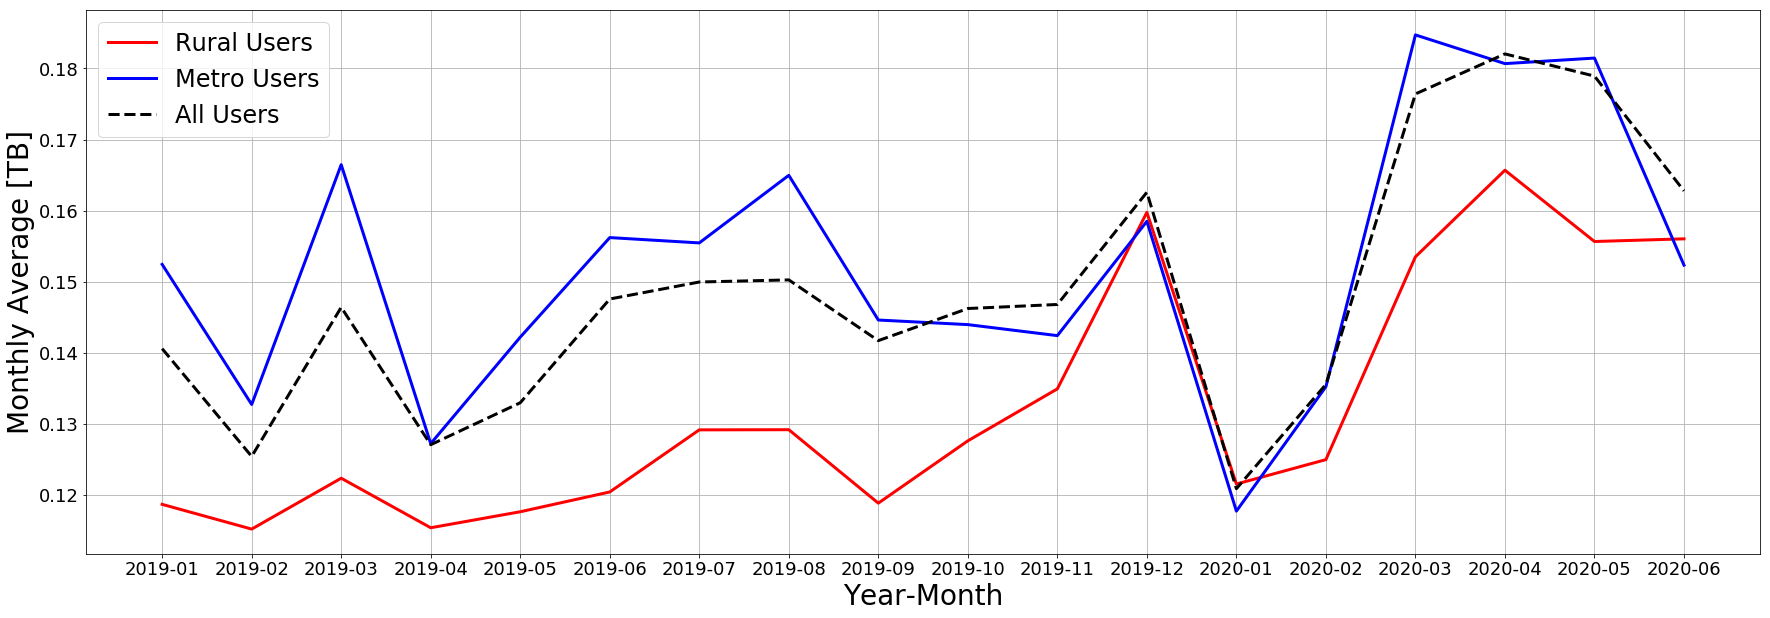
\includegraphics[width=1.0\linewidth]{figs/monthly_downloaded_data_notitle.png}
    \caption{Graph showing the monthly average downloaded data per user from January 2019 to June 2020, partitioned by test unit county population.}
    \label{fig:downloadmetro_rural}
\end{figure*}

\begin{figure*}[t]
    \centering
    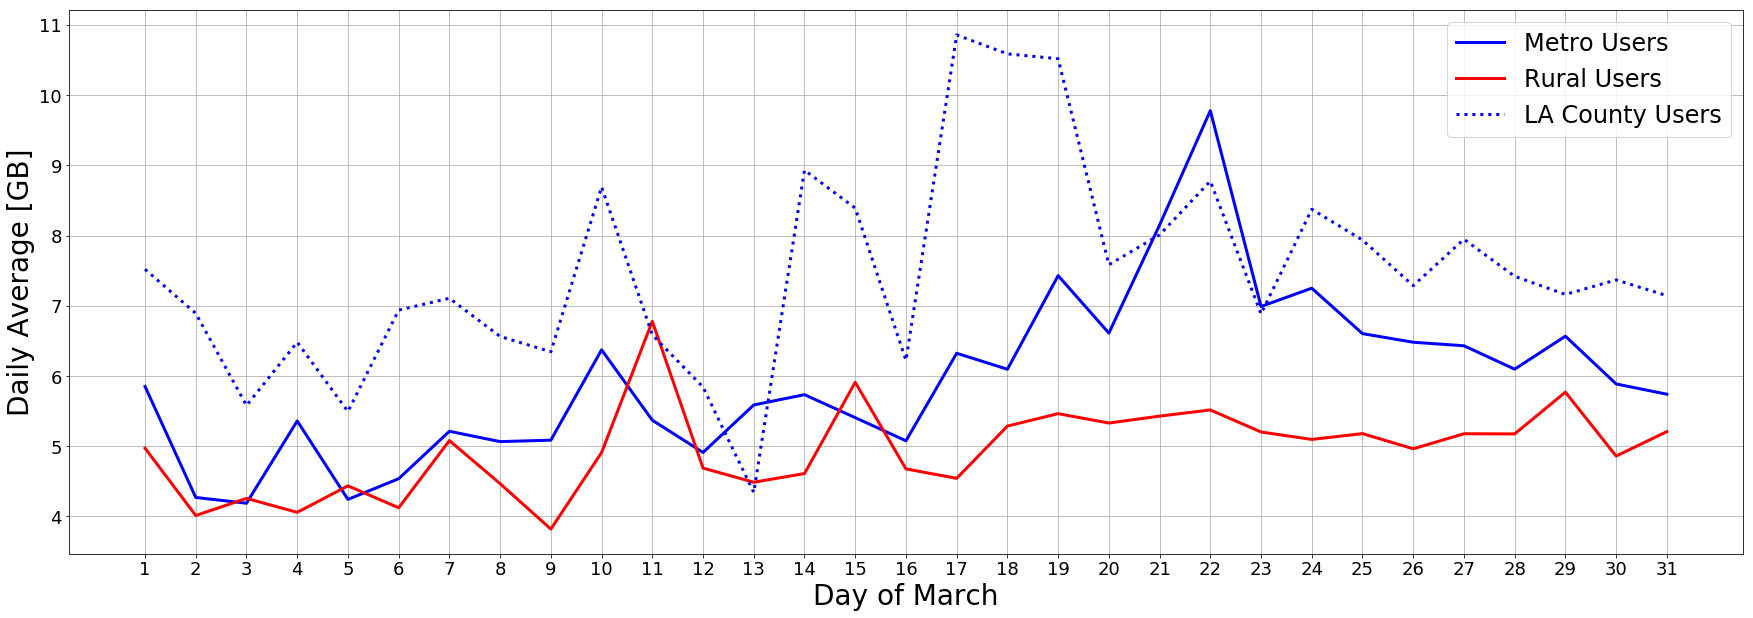
\includegraphics[width=1.0\linewidth]{figs/daily_downloaded_data_notitle.png}
    \caption{Graph showing the daily downloaded data per user in March 2020 for those in metro and rural areas, as well as LA county.}
    \label{fig:dailymetro_rural}
\end{figure*}

\section{Data Usage by Population Demographics}
\label{sec:data-usage-by-population-demographics}

\subsection{Average Monthly Downloads}

A high-level overview of the effect of COVID-19 on fixed broadband internet usage can be seen by analyzing the average monthly downloaded data per user. As can be seen in Figure \ref{fig:downloadmetro_rural}, we notice a sizable increase in overall downloaded data in the months of March, April, and May 2020. This increase is consistent across both metro and rural counties, although it is more pronounced in metro areas. The three pandemic months are the highest-usage months for metro areas. In contrast, rural areas only have one month larger than their pre-pandemic maximum of December 2019. 

Interestingly, in the fourth month of the pandemic, we notice a drop in overall downloaded data in metro areas, while rural areas remain constant. This drop coincides with the relaxation of many stay-at-home orders, indoor dining bans, and curfews in cities across the United States \cite{money2020la,gov2020nyc}. 

% \begin{figure*}
%     \centering
%     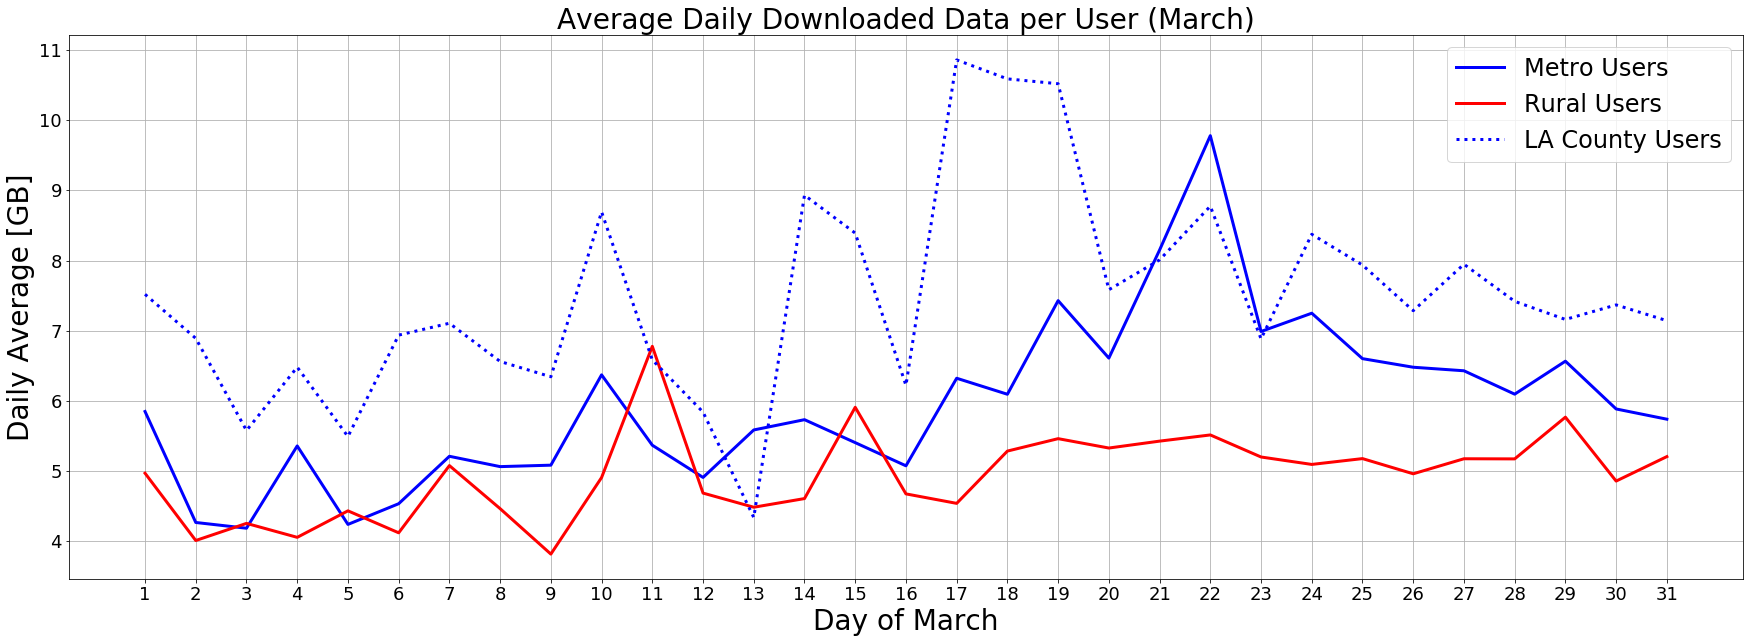
\includegraphics[width=1.0\linewidth]{figs/daily_downloaded_data.png}
%     \caption{Graph showing the daily downloaded data per user in March 2020 for those in metro and rural areas, as well as LA county.}
%     \label{fig:dailymetro_rural}
% \end{figure*}

\subsection{Average Daily Downloads}
Focusing on daily fixed broadband internet usage can allow us to understand the public's reactions to various events. In particular, by analyzing daily overages over the course of March, we can better understand the reactions to the various stay-at-home orders, school shutdowns, and curfews from an internet usage point-of-view. 

To this end, we present in Figure \ref{fig:dailymetro_rural} the daily average downloaded data usage for both metro and rural users. The first event we look to analyze is the White House first announcing its social distancing recommendations on March 16 for the entire country \cite{trump2020coronavirus}. Following this announcement, we observe that users in metro areas use a significantly larger amount of data than those in rural areas. In the first half of the month, there was no such difference (Figure \ref{fig:dailymetro_rural}). It is unsurprising that those in cities and other metro areas reacted to this recommendation more drastically than those in less populated areas. Cities such as New York City, San Francisco, and Los Angeles (LA) were among the hardest hit areas in the early weeks of the pandemic \cite{cdc2020tracker}. 

For many of the aforementioned cities, various levels of lockdowns were put in place on top of the White House's recommendations \ref{tab:state-lockdown}. Therefore, we additionally investigate if we can correlate these local ordinances with county-level usage patterns. Los Angeles (LA) county has the most test units in the FCC MBA dataset ($n=44$), so we examine the daily average downloaded data per user for all those residing in LA (Figure \ref{fig:dailymetro_rural}). 

We observe the first large spike on March 14, the day after many schools in the county shutdown \cite{haire2020LA}. March 14 was a Saturday, so this spike is not due to remote learning. However, if schools were shut down by this date, then we can reasonably expect that various other aspects of society were shut down. For example, although the official order to ban indoor dining came later, by March 14, many LA restaurants were were already closed\cite{eater2020}. This would suggest that the spikes we observe following government orders are due to people seeking entertainment from the internet over outside options.

We also notice a larger spike in the days following the March 16 White House stay-at-home order. 
\subsection{The Data Consumption}
\label{sec:the-data-consumption}
In this sub-section we present the results that show how COVID-19 changed the amount of average data downloaded and uploaded per user.

\subsubsection{Data Downloaded}
\label{sec:download-data-consumption}

In order to analyze the impact of COVID-19 on the amount of data downloaded, we calculated the average consumption per user and per month in the timeline of January-March 2020. After the averages were computed, Figure \ref{fig:download2020} was generated and it shows how the average amount of data downloaded per user has changed from January to March.

\begin{figure}
\centering
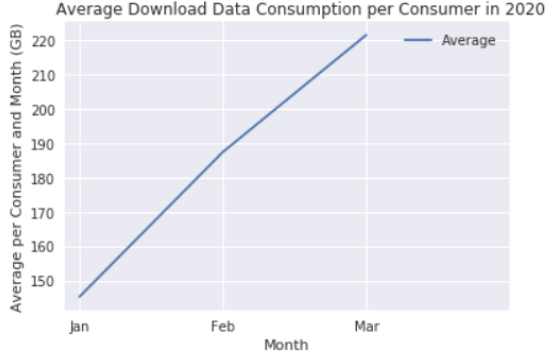
\includegraphics[width=1.0\linewidth]{figs/download2020.PNG}
\caption{Graph showing the average consumption of downloaded data per user for the first three months of 2020.}
\label{fig:download2020}
\end{figure}

As Figure \ref{fig:download2020} shows, in January the average amount of data downloaded per consumer was approximately \SI{145}{\giga\byte} and in March this value went up to approximately \SI{221}{\giga\byte}. This shows that from January to March there was an increase of approximately \SI{53}{\percent} in the average per consumer. Figure \ref{fig:downloadup2019} shows the average of data downloaded and uploaded per user from January to March 2019. As the graph shows, in 2019 from January to March there was actually a decrease in the value of data downloaded (average for download is represented by the red line). Thus, one could conclude that the trend in data downloaded per user changed from 2019 to 2020, since instead of decreasing, the average per consumer increased considerably from January to March in 2020. Therefore, it is possible to conclude that this new trend in the quantity of data downloaded was established due to the COVID-19 outbreak as this was the strongest external factor that influenced Internet usage in the US in the first semester of 2020. In addition to that, as people stayed at home more in March, one possible explanation for this change in the value of downloaded data could be that they spent more time with online entertainment, e.g., video streaming services and games and also watching their classes from their computers, making their average amount of data downloaded to go up and showing that people tended to comply with stay at home orders.

\begin{figure}
\centering
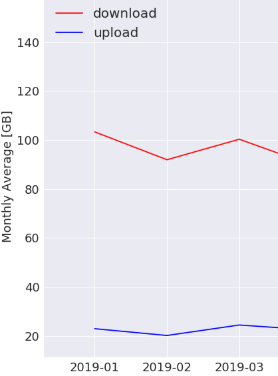
\includegraphics[width=0.5\linewidth]{figs/downloadup2019.PNG}
\caption{Graph showing the average consumption of downloaded and uploaded data per user for the first three months of 2019.}
\label{fig:downloadup2019}
\end{figure}

\subsubsection{Uploaded Data}
\label{sec:upload-data-consumption}

Similarly to the average downloaded data analysis, while computing the average amount of data uploaded per consumer for the period of January-March of 2020, we could observe an increase in the average value from January to March. Figure \ref{fig:upload2020} is the graph for the average amount of data uploaded per consumer in the first three months of 2020 and shows that in January the average consumption per consumer (called in the graph as Unit-id) was approximately \SI{25}{\giga\byte} while in March it increased to approximately \SI{37}{\giga\byte}. These numbers show that there was an increase in the average value of data uploaded per consumer of approximately \SI{38}{\percent}. Moreover, Figure \ref{fig:downloadup2019} also shows the average of uploaded data per consumer in 2019. According to the graph (average for upload is represented by the blue line), in 2019 there was a small increase in the average data uploaded per consumer from January to March. However, this increase was less than \SI{2}{\percent} showing an increase not as relevant as the increase observed between the same months in 2020. Hence, it is possible to conclude that there was also a shift in the trend of the average data uploaded per consumer from January to March comparing 2019 and 2020. Moreover, as the increase in the average in 2020 was approximately 19 times bigger than the increase in 2019, it is clear that COVID-19 also impacted the average amount of data uploaded per user, considering that this was the external factor that impacted the consumption of Internet as a whole in 2020.

\begin{figure}
\centering
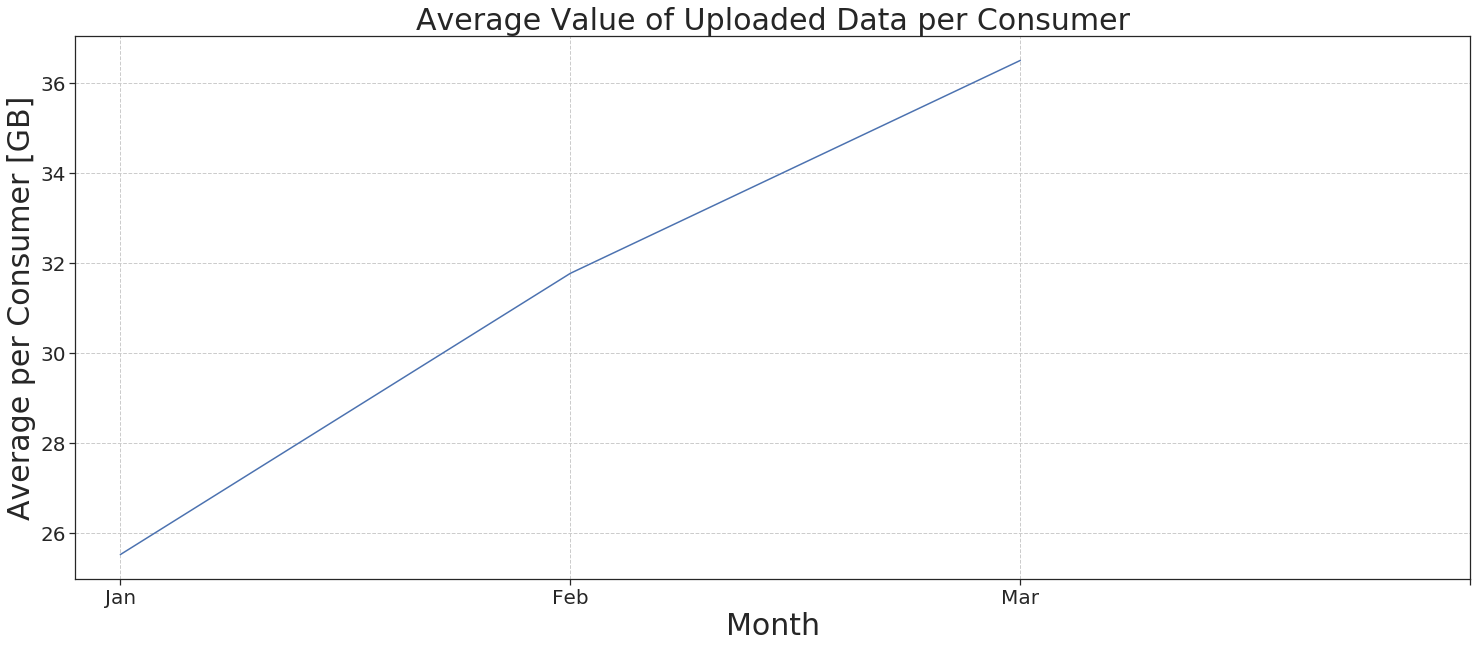
\includegraphics[width=1.0\linewidth]{figs/upload2020.PNG}
\caption{Graph showing the average consumption of uploaded data per user for the first three months of 2020.}
\label{fig:upload2020}
\end{figure}

Therefore, it can be concluded that the COVID-19 changed Internet usage in the US in the first quarter of 2020. The increase in the averages of data downloaded and uploaded per consumer from January to March in 2020 explicitly shows that there was an outside event that impacted the usage of Internet making it higher than it would be expected based on the trends of Internet consumption established from January to March of 2019. Since there was not any other major event influencing  Internet usage in March 2020, it is possible to conclude that this increase in the average amount of data downloaded and uploaded happened due to COVID-19, since people were using Internet more while they were complying to stay at home orders and quarantining.

\subsection{Average Speed}

% \begin{figure*}[t]
%   \centering
%   \includegraphics[width=.49\textwidth]{figs/wenjun/test.png}
%   \includegraphics[width=.49\textwidth]{figs/wenjun/test.png}
%   \centering
%   \includegraphics[width=0.5\textwidth]{figs/wenjun/download_compare.png}

%   \begin{scriptsize}\hspace*{-1em}
%   \begin{tabular}{l}
%     TODO
%   \end{tabular}
%   \end{scriptsize}
%   \vspace*{-1em}
%   \caption{caption: TODO.}
%     \vspace*{-1em}
%   \label{fig:top1-scores}  
% \end{figure*}

\label{sec:average-speed}
Besides analyzing the average amount of data downloaded and uploaded per consumer in 2020, we also analyzed how the average speed experienced by consumers changed due to COVID-19. By knowing that the average value of data used per user increased significantly, it could be expected a change in the average speed that people experienced in the middle of quarantine, since ISPs could not be ready to adapt and supply the same average speed to all users, considering the expressive increase in data downloaded and uploaded.

\subsubsection{Average Download Speed}
\label{sec:average-download-speed}

In order to understand how the COVID-19 outbreak impacted the average download speed experienced by consumers, we calculated the ratio between the average download speed that users had access to in January and March 2020. The ratio was computed by the following formula:

\begin{equation}
ratio= ((av.speed.Mar - av.speed.Jan)/ av.speed.Jan)*100
\end{equation}

Figure \ref{fig:downloadspeed2020} shows the results of the compilation of the ratios in a CDF format and, according to this graph, it is possible to infer that approximately \SI{70}{\percent} of the users experienced a decrease in their average download speed from January to March. This is not the finalized version of the graph yet, since considering how noisy and big the data set is, it is indeed tough to process all the data and find the final version of the graphs. However, Figure \ref{fig:downloadspeed2020} already shows reliable results if we compare them to what other studies related to the topic have shown as they show that indeed the average download speed decreased during March 2020. It is also important to note that while approximately \SI{80}{\percent} of the users experienced a decrease in their download speed, this decrease was a modest value of few percentages. In the article \textit{ Internet Speed Analysis: Top 200 Cities, March 15th – 21st} \cite{cooper}, Cooper affirms that although some ISPs were able to hold up the increase in  Internet consumption, some cities felt the impact of the increase in data consumption leading users to experience a decrease in their download speed, e.g., the download speed in New York City decreased by \SI{24}{\percent} in March. This decrease in the average download speed in some cities is a result of the decrease of average download speed that consumers have experienced from January to March in 2020 and vice-versa.

\begin{figure}
\centering
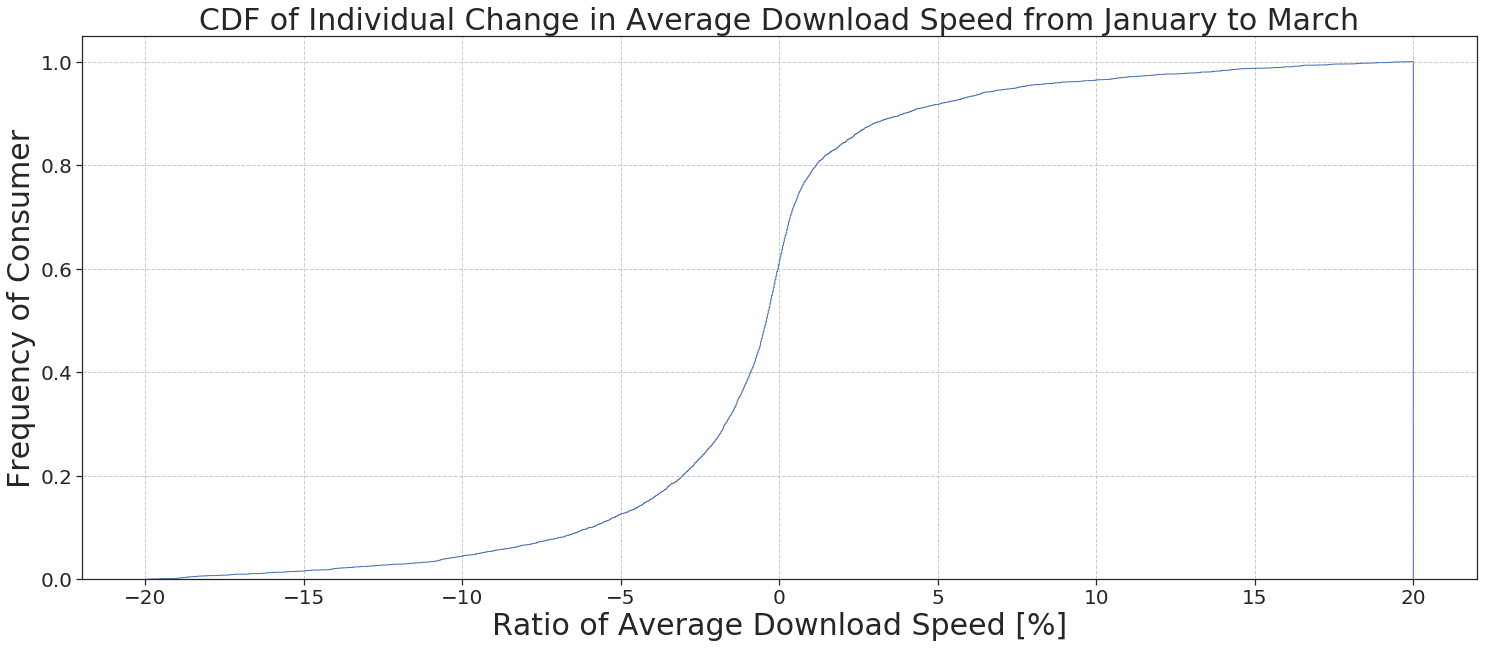
\includegraphics[width=1.0\linewidth]{figs/downspeed.PNG}
\caption{CDF that shows the ratios of average download speed experienced per consumer between January and March of 2020.}
\label{fig:downloadspeed2020}
\end{figure}

\subsubsection{Average Upload Speed}
\label{sec:average-upload-speed}
Similarly to the average download speed, we also computed the ratio between the average upload speed experienced by users in January and March 2020. The formula used was similar to the ratios for average download speed and can be represented by the following:
\begin{equation}
ratio= ((av.speed.Mar - av.speed.Jan)/ av.speed.Jan)*100
\end{equation}

Figure \ref{fig:uploadspeed2020} shows the compiled result of these ratios and, according to this graph, approximately \SI{80}{\percent} of consumers (called unit-ids in the graph) saw their average upload speed decreasing from January to March 2020. As people transitioned most of their activities to a virtual environment, such as working and studying from home and had to log in calls and virtual conferences more often, it could be expected an increase in data upload (as Figure \ref{fig:upload2020} shows) and, consequently, a decrease in the average upload speed, since there were more data being uploaded than before. Again, similarly to the situation observed with the download speed, while \SI{80}{\percent} of consumers experienced a decrease in their upload speed, this decrease was also modest of just a few percentages.

\begin{figure}
\centering
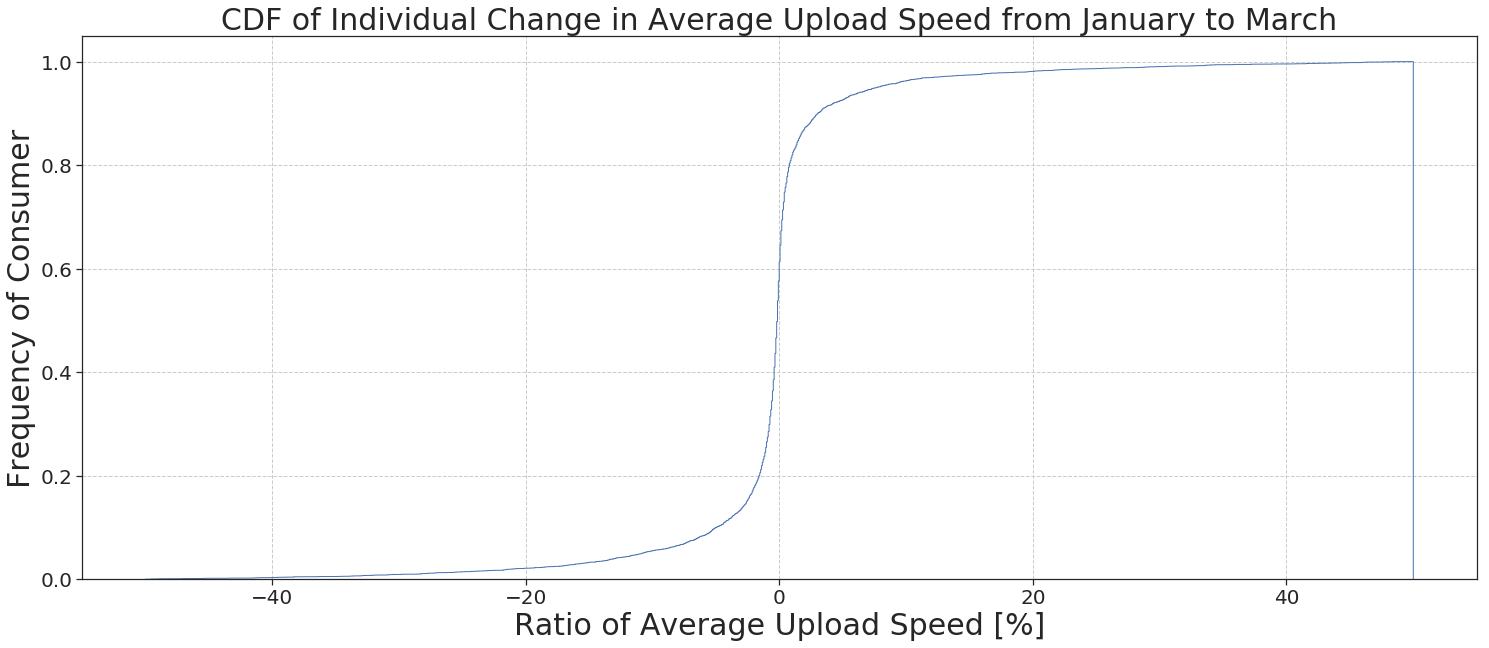
\includegraphics[width=1.0\linewidth]{figs/uploadspeed.PNG}
\caption{CDF that shows the ratios of average upload speed experienced per consumer between January and March of 2020.}
\label{fig:uploadspeed2020}
\end{figure}

\subsection{Consumers with the heaviest Internet consumption}
\label{sec:analyzing-the-users-with-the-highest-internet-usage}

One component analyzed in this research was how the users who extensively used Internet before the pandemic, have been using it after the COVID-19 outbreak. This analyzes hopes to gain more behavioral insights about people's Internet consumption. Thus, we identified the \SI{10}{\percent} of users (approximately 500 users) who had the highest averages of data downloaded and uploaded and computed the ratio of average usage between January and March in order to find out if their usage increased or decreased after COVID-19 hit the country in early March.

\subsubsection{Heavy Download Users}
\label{sec:heavy-download-users}

In order to analyze the data usage of only heavy users, we computed the ratio of data downloaded between January and March for users who downloaded more than \SI{400}{\giga\byte} in January, in order words: we computed the ratios of data downloaded for approximately \SI{10}{\percent} of the users who downloaded the most data in January. We applied the following formula to calculate the ratios:
\begin{equation}
ratio= data.downloaded.Mar/ data.downloaded.Jan
\end{equation}

After computing the ratios for the \SI{10}{\percent} of users who downloaded the most data in January, we computed the CDF shown in Figure \ref{fig:heavydown}.

\begin{figure}
\centering
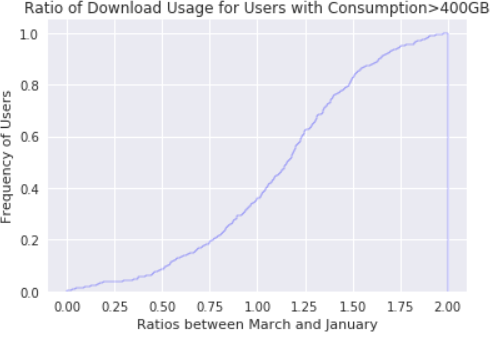
\includegraphics[width=1.0\linewidth]{figs/heavydown.PNG}
\caption{CDF that shows the ratios of average amount of data downloaded per consumer between January and March 2020 for consumers who downloaded more \SI{400}{\giga\byte} in January (top \SI{10}{\percent} of consumers for data downloaded in January).}
\label{fig:heavydown}
\end{figure}

The graph shows that approximately \SI{40}{\percent} of the users decreased or did not change their consumption of data downloaded. While this number was expected to be bigger, considering that before quarantine and stay at home orders took place these users were already using  Internet on its maximum capacity, a possible explanation to an increase in Internet consumption for this users is that possibly during quarantine, they spent even more time using video streaming service, e.g., Netflix and YouTube. According to Kovacs \cite{kovacs}, the world suffered from a more extensive Internet traffic in March which was primarily caused by video streaming services. Kovacs also explained in her paper \textit{U.S. broadband networks rise to the challenge of surging traffic during the pandemic} that \SI{24}{\percent} of  Internet traffic in the US was caused by video services and that as a response, in March Netflix reduces its streaming speed and YouTube only allowed standard definition on its videos worldwide.

\subsubsection{Heavy Upload Users}
\label{sec:heavy-upload-users}

We also computed the ratios of data uploaded between January and March for \SI{10}{\percent} of the users who uploaded the most data in January. This analysis included approximately 500 users who uploaded more than \SI{47}{\giga\byte} in January. The formula used to calculate the ratios was similar to the one used for heavy download users and can be represented by:

ratio=upload bytes used in March / upload bytes used in January

After computing the ratios for the \SI{10}{\percent} of users who uploaded the most data in January, we generated the CDF shown in Figure 7. According to the graph, \SI{60}{\percent} of users decreased or did not change their consumption for January to March. As this represents most of the heavy the users, a possible explanation for this decrease/no change in uploaded data by their consumers could be that when COVID-19 hit the country back in late February, people had to relocate, many left the big cities of the country and college campuses to return to their homes in the suburbs. By migrating, these people could possibly relocate in an area in which they could have had a bad Internet connection and or more options of outdoor activities, such as hiking. This who led them to not use  Internet as intensively as they were using before.

Moreover, another possible explanation for those who experienced no change in their download data consumption could be that as they were already consuming in their maximum capacity, when the stay at home orders took place, these people did not change their Internet consumption that much, since they were already consuming as much as they could before quarantining. It is also interesting to see that \SI{40}{\percent} of the heavy upload users increased their consumption of uploaded data. Although this was not expected, a possible explanation for this increase is that with the quarantine and lock-down policies taking place, people started working from home and participating in more video conferences. By logging in Zoom meetings and other video conference services more frequently, their consumption of upload bytes increased significantly from January to March.
\begin{figure}
\centering
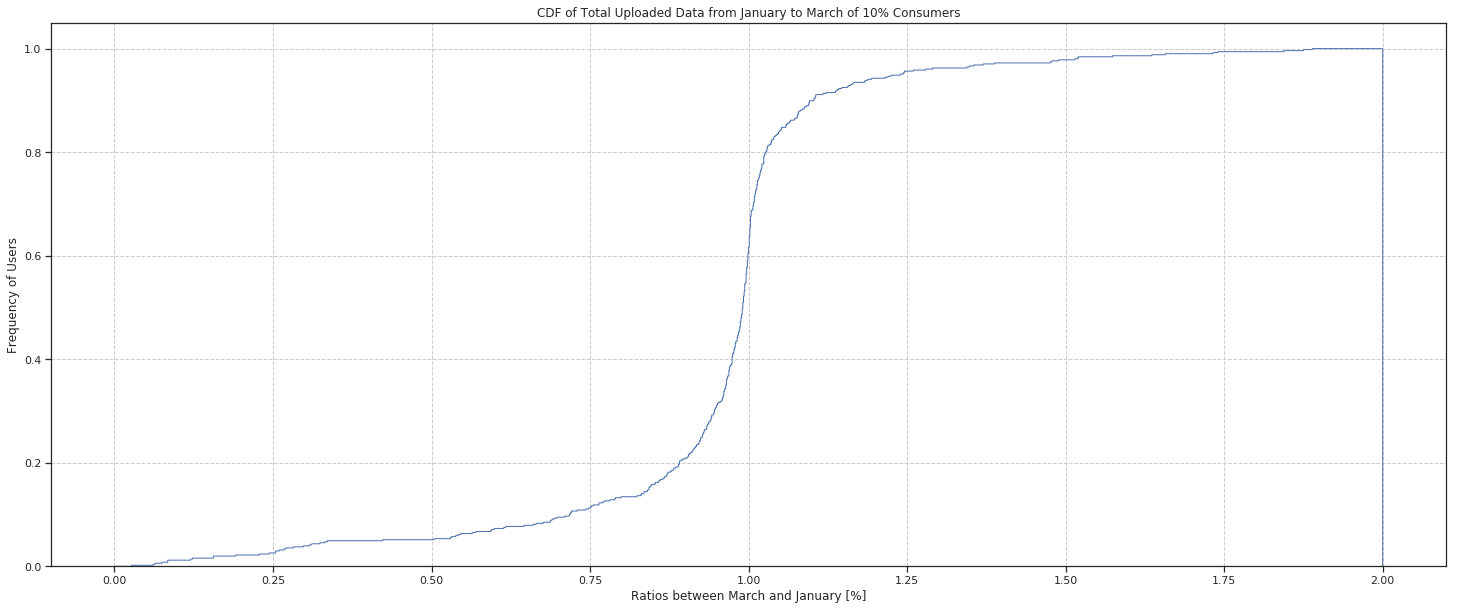
\includegraphics[width=1.0\linewidth]{figs/heavyup.PNG}
\caption{CDF that shows the ratios of average amount of data uploaded per consumer between January and March 2020 for consumers who uploaded more \SI{47}{\giga\byte} in January (top \SI{10}{\percent} of consumers for data downloaded in January).}
\label{fig:heavyup}
\end{figure}

% wenjunchen
\subsection{Average Data Usage per Users over Hours on Each Month}
We study the average data usage per users over hours on each month by comparing the average data usage on weekdays or weekends, and before COVID-19 or after COVID-19 based on both download data and upload data. Since the recorded time in data set is finished in coordinated universal time, in order to get the time of download or upload event at local time, we add the time zone offset from the user profile to the recorded time.  We extract the year, month, and hour from the local time, and handle some special cases: (1) for hour, there is some location behind coordinated universal time and if the hour in local time is negative, add the value by 24. (2) For month, if the value of hour in local time is negative and the day is 1, we subtract the value of extracted month by 1 because it will be the last date of the previous month, and (3) for year, if the value of hour in local time is negative, the month is 1 and the day is 1, we subtract the value of extracted year by 1 since it will be the last date of the previous year. For the users, we focus on users who are present throughout the course of the study. We notice that the number of bytes that the customer transmitted from wired LAN devices to the internet for some users is the value of maximum integer. The possible reason is that the device measuring that value may be broken so we ignore all the users who have those values. 

% Downloaded MB
\begin{figure*}[t]
  \centering
  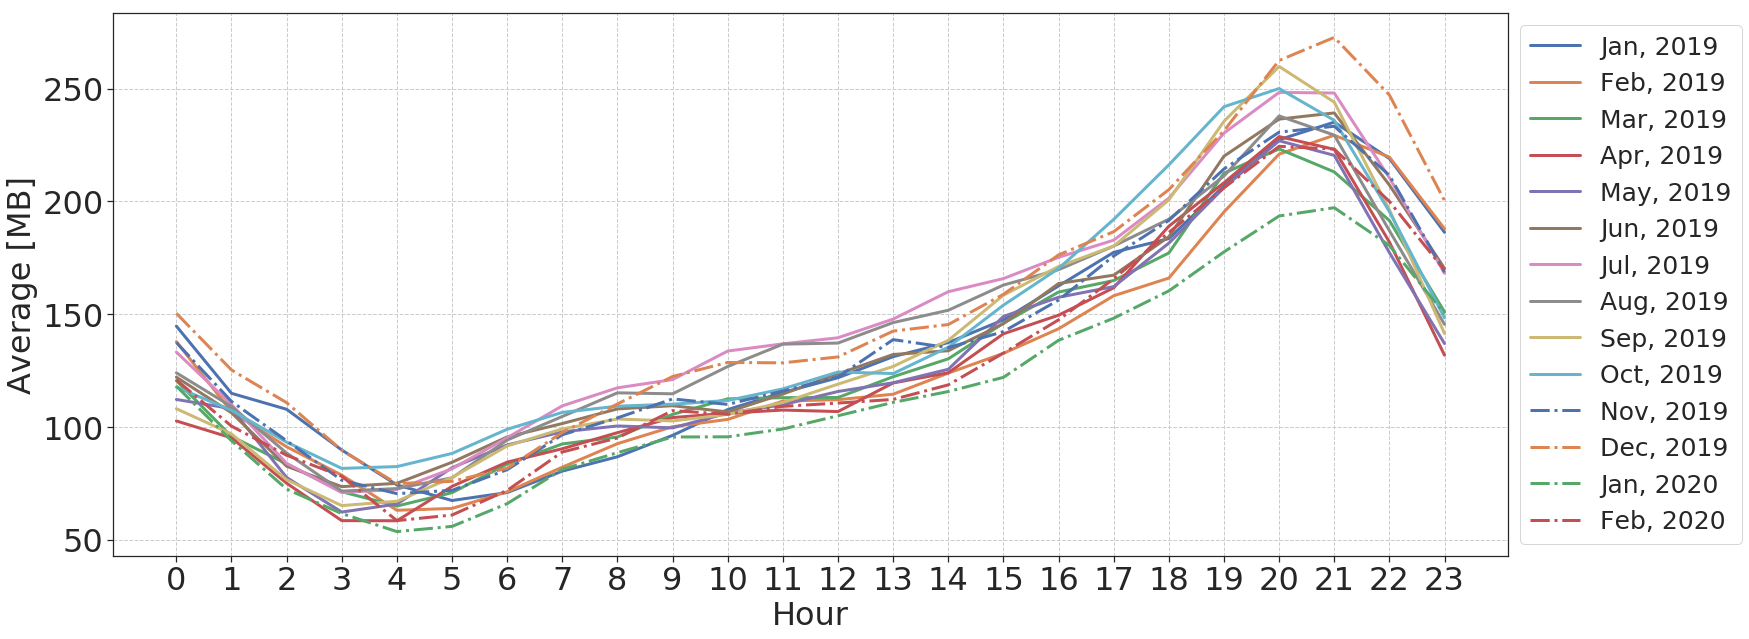
\includegraphics[width=.49\textwidth]{figs/wenjun/download_wdays_before.png}
  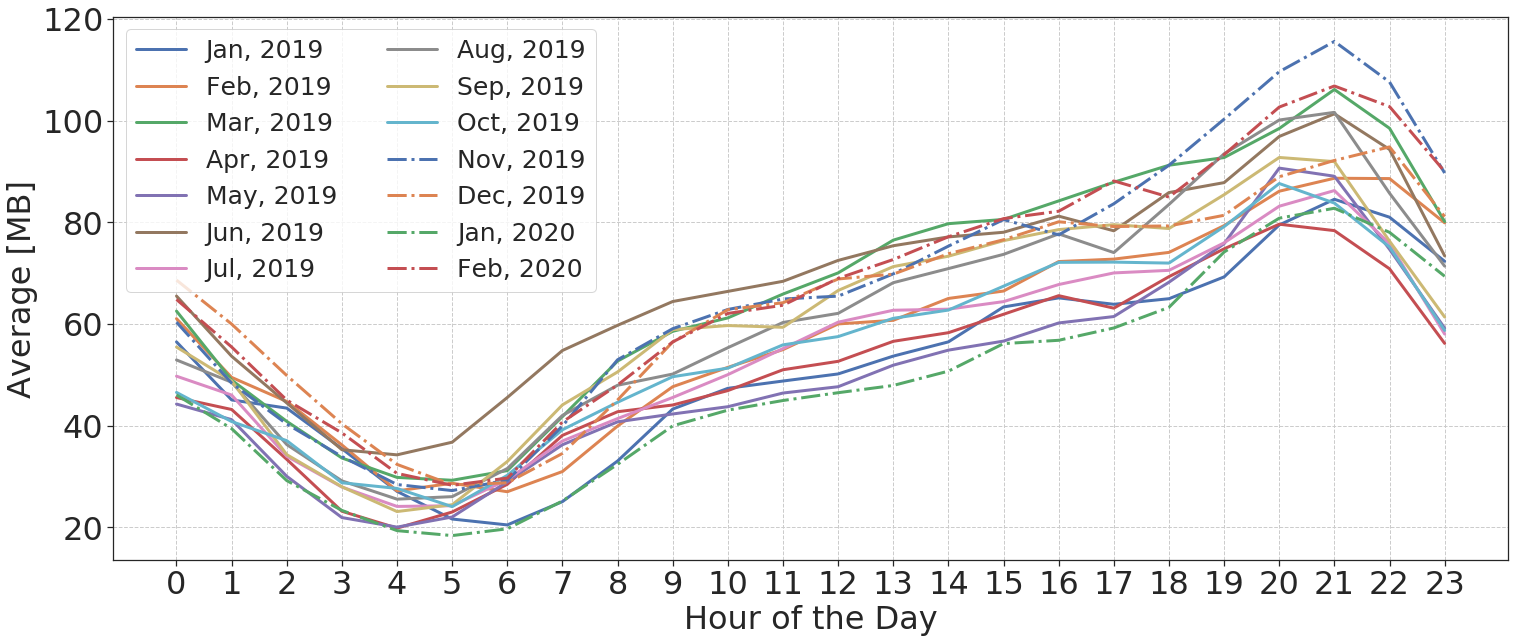
\includegraphics[width=.49\textwidth]{figs/wenjun/download_wends_before.png}
  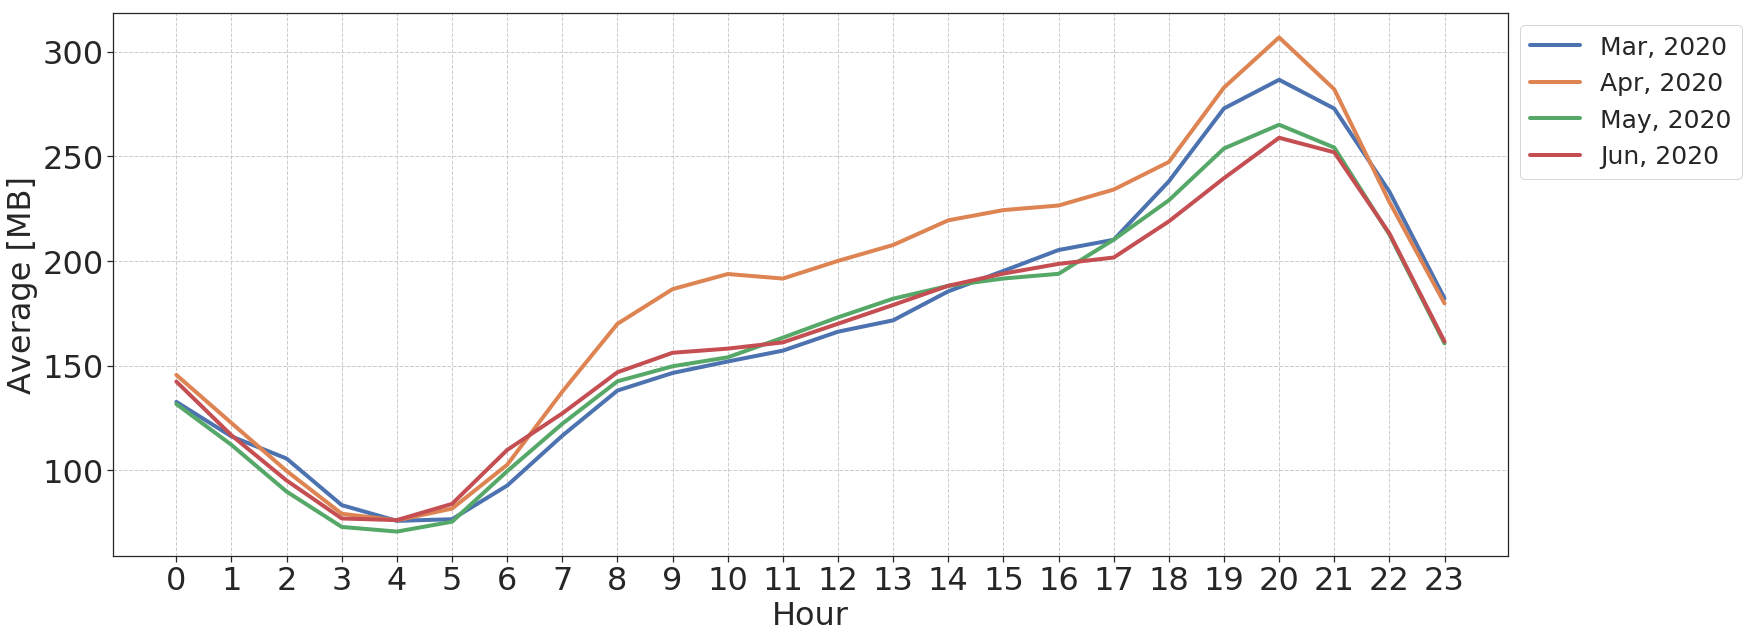
\includegraphics[width=.49\textwidth]{figs/wenjun/download_wdays_after.png}
  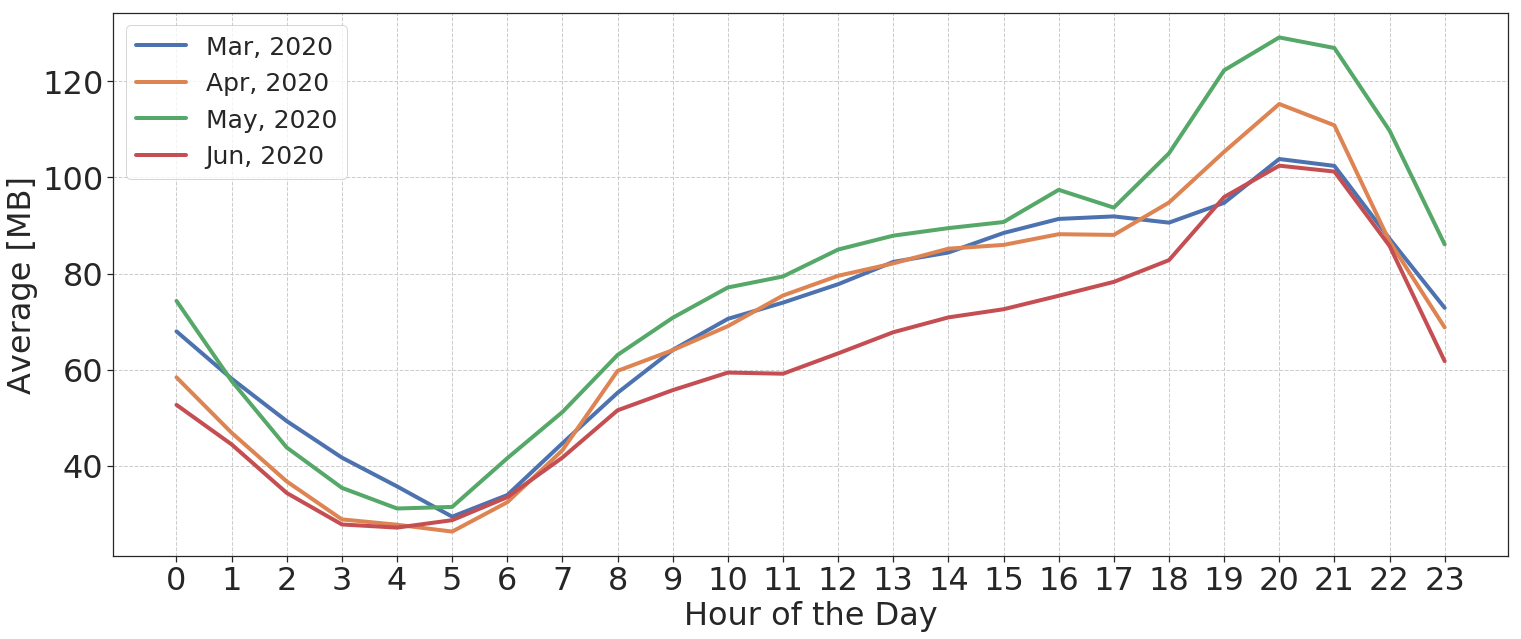
\includegraphics[width=0.49\textwidth]{figs/wenjun/download_wends_after.png}
  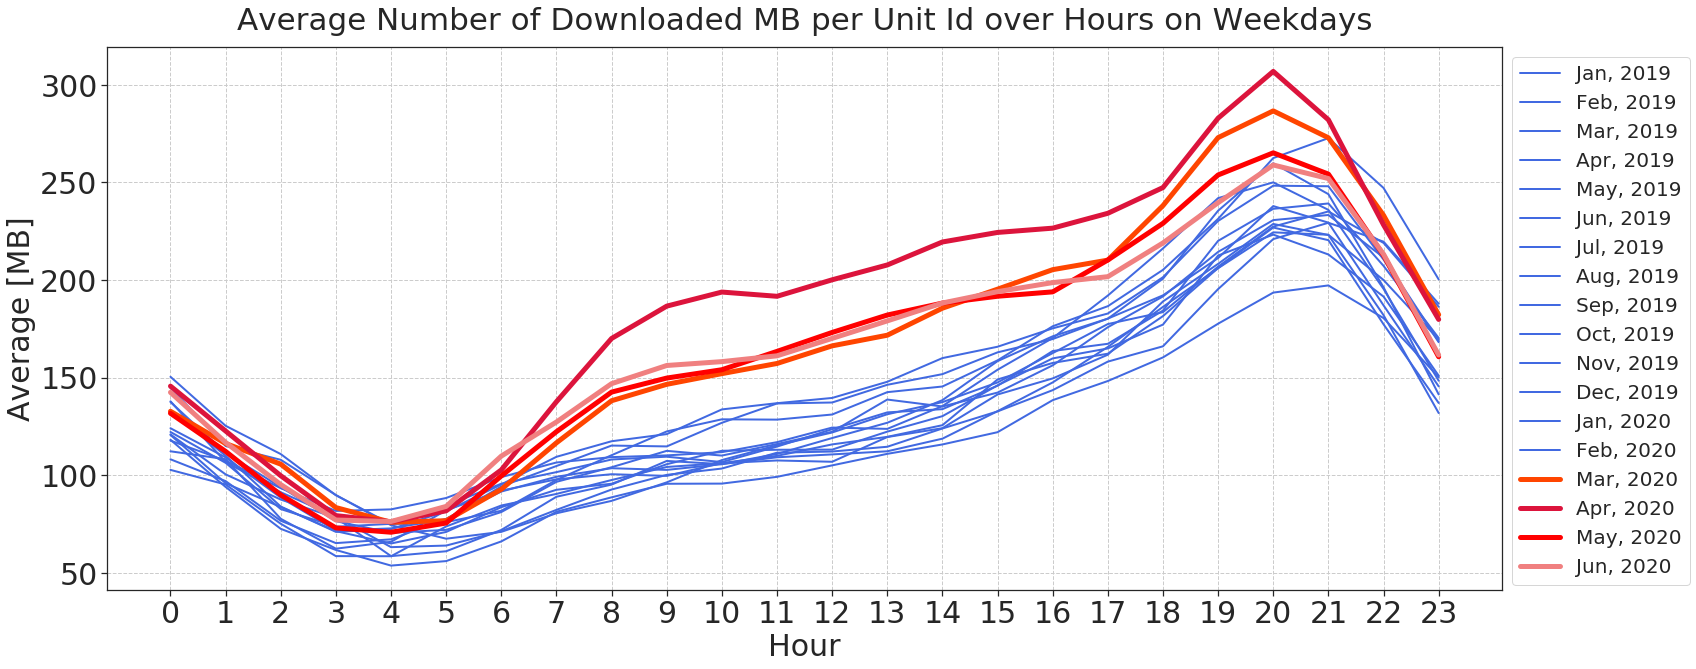
\includegraphics[width=.49\textwidth]{figs/wenjun/download_wdays_compare.png}
  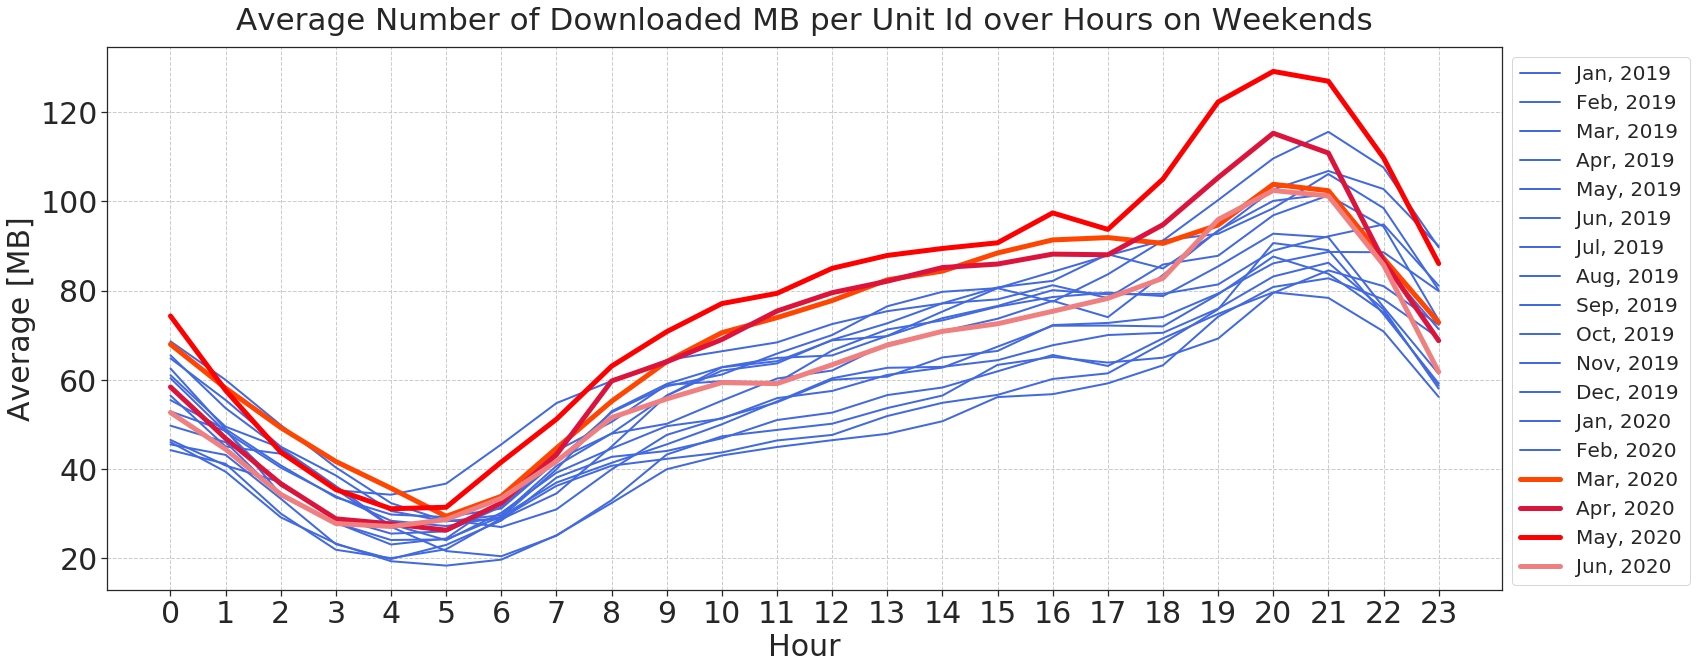
\includegraphics[width=0.49\textwidth]{figs/wenjun/download_wends_compare.png}

  \vspace*{-1em}
  \caption{TODO: Download data.}
    \vspace*{-1em}
  \label{fig:download-data-per-user-hours-fig}  
\end{figure*}

\subsubsection{Average Download Data per User}
\label{sec:download-data-per-user-over-hours}

The download data is the number of bytes that the customer received from the internet to wired LAN devices and the Wi-Fi devices. As shown in the Figure \ref{fig:download-data-per-user-hours-fig}, we can find that the patterns of download data usage are the same on weekdays and weekends whether before COVID-19 or after COVID-19. There is a peak between 18:00p.m. and 22:00p.m. \textbf{(TODO: why people always use more internet after dinner? Entertainment? Need more research)}

Moreover, according to the two graphs at the third row in Figure \ref{fig:download-data-per-user-hours-fig}, the average download data per user over hour after COVID-19 (red) is larger than that before COVID-19 (blue). On weekdays, the gaps between red lines and blue lines from 8:00 a.m. to 22:00 p.m. are more obvious that those from 22:00 p.m. to 8:00 a.m. next day. The increase from 8:00 a.m. to 18:00 p.m. may be because of work from home or online courses, and the increase from 18:00 p.m. to 22:00 p.m. may be because people can not hangout with their friends or have less outdoor activities because of social distancing and quarantine. Instead, people need to stay at home and may watch movie, play video games, and so on. Besides, people have poorer efficiency because of quarantine, and they may need more time to finish their work after dinner as well. \textbf{(TODO: need reference)} From 22:00 p.m. to 8:00 a.m. next day, it is time for rest so the average number of download data per user after COVID-19 does not have too much difference with that before COVID-19. On weekends, the difference between red lines and blue lines at daytime is not that obvious but the gap from 18:00 p.m. to 22:00 p.m. is still pretty larger, especially on May \textbf{(TO DO: why May?)}. People have a rest on weekends, so the usage of internet is less at daytime. After dinner, people need internet for their entertainment time. Therefore, we can conclude that people use more internet and download more data after COVID-19.

% Uploaded MB
\begin{figure*}[t]
  \centering
  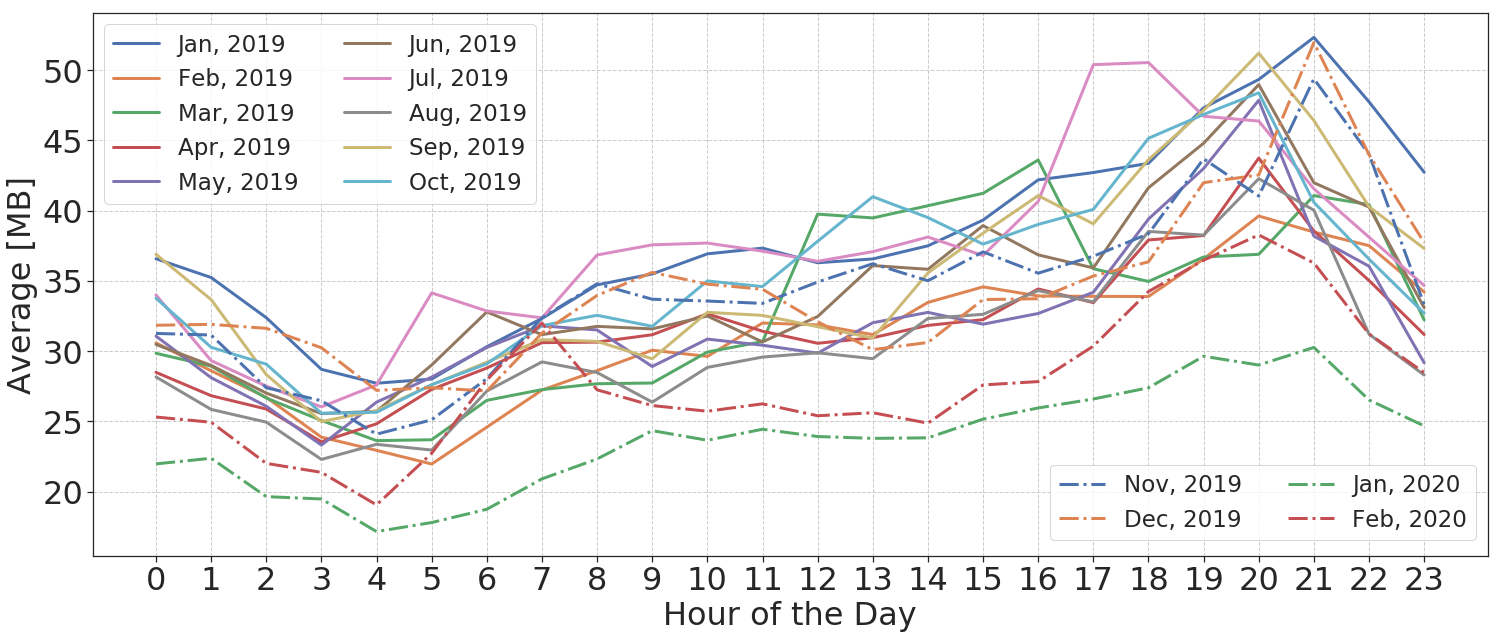
\includegraphics[width=.49\textwidth]{figs/wenjun/upload_wdays_before.png}
  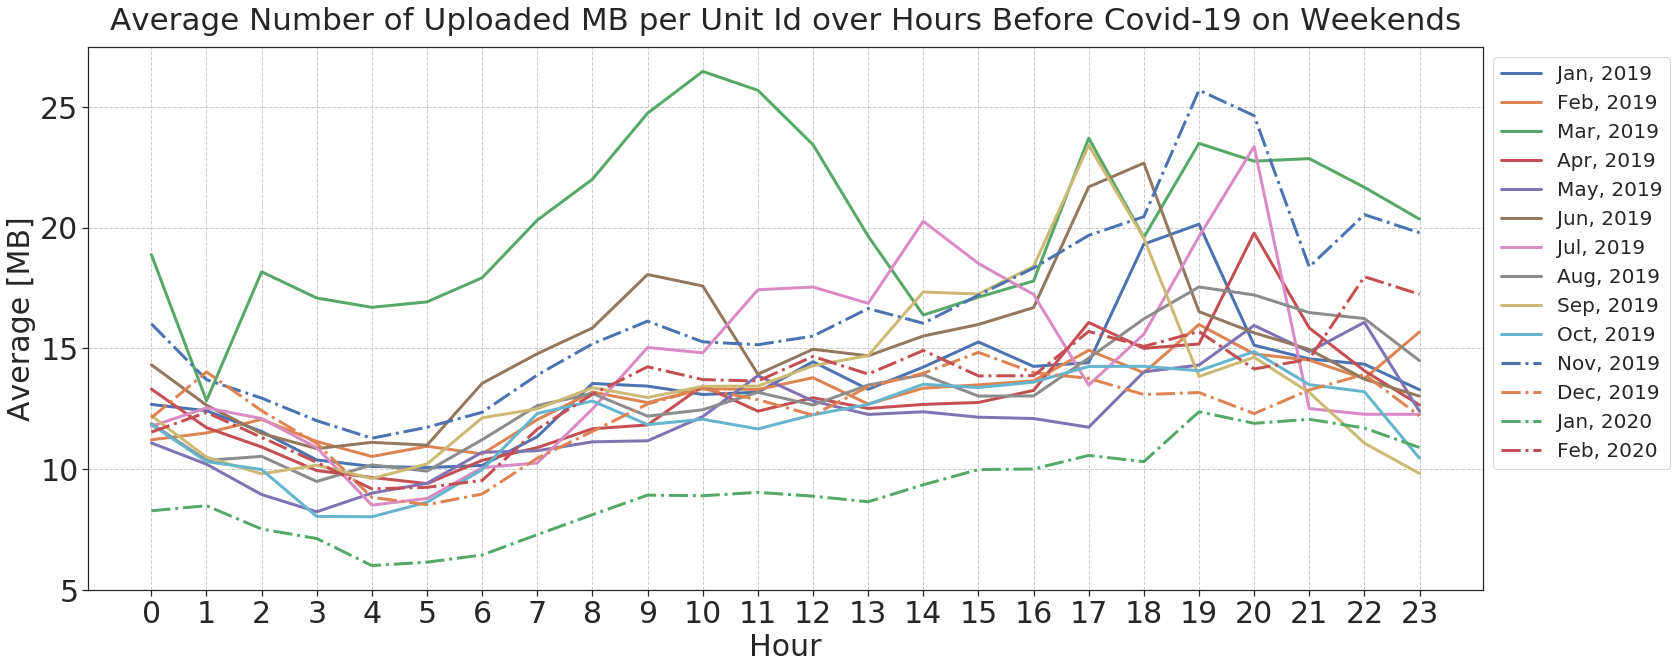
\includegraphics[width=.49\textwidth]{figs/wenjun/upload_wends_before.png}
  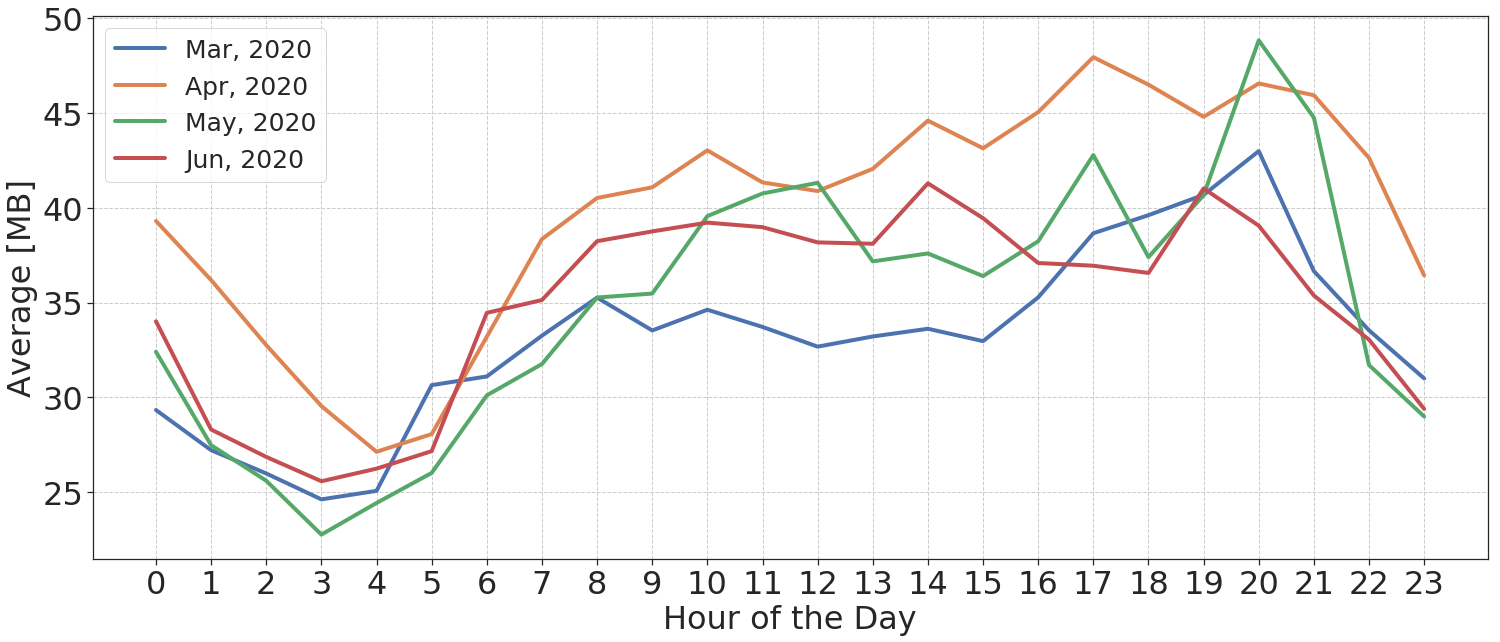
\includegraphics[width=.49\textwidth]{figs/wenjun/upload_wdays_after.png}
  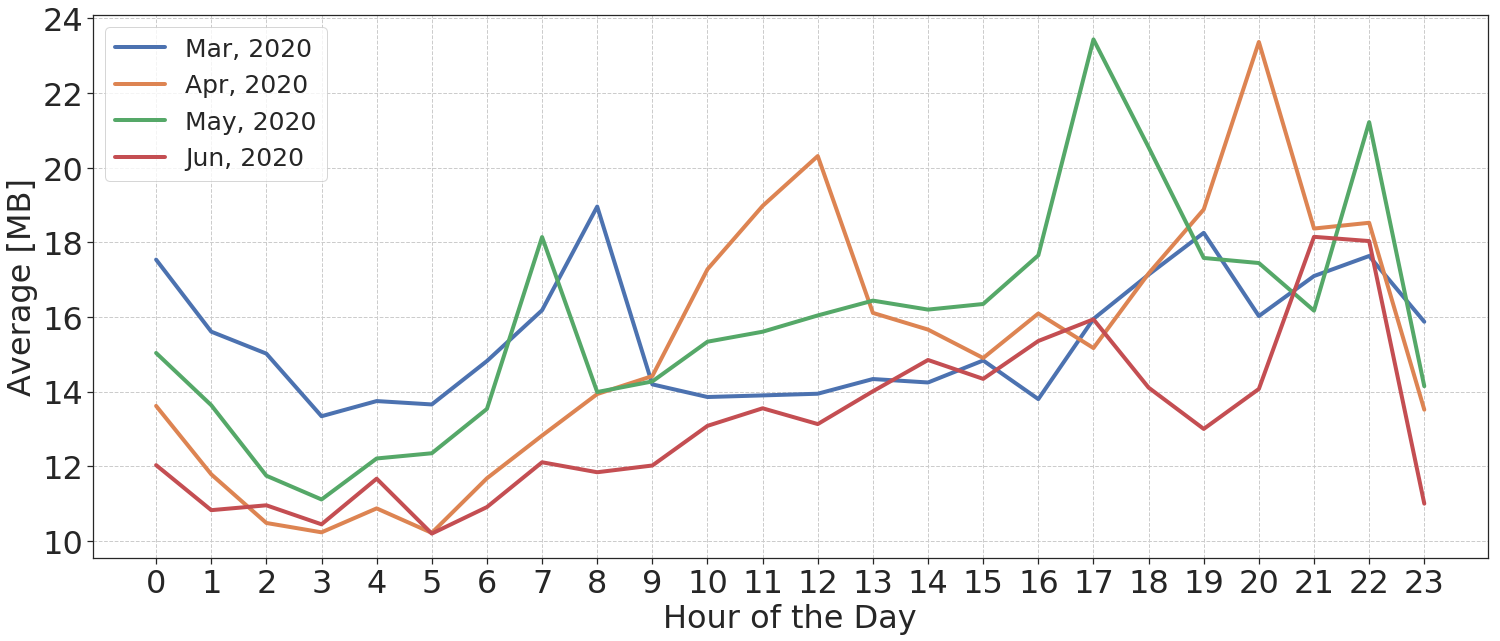
\includegraphics[width=0.49\textwidth]{figs/wenjun/upload_wends_after.png}
  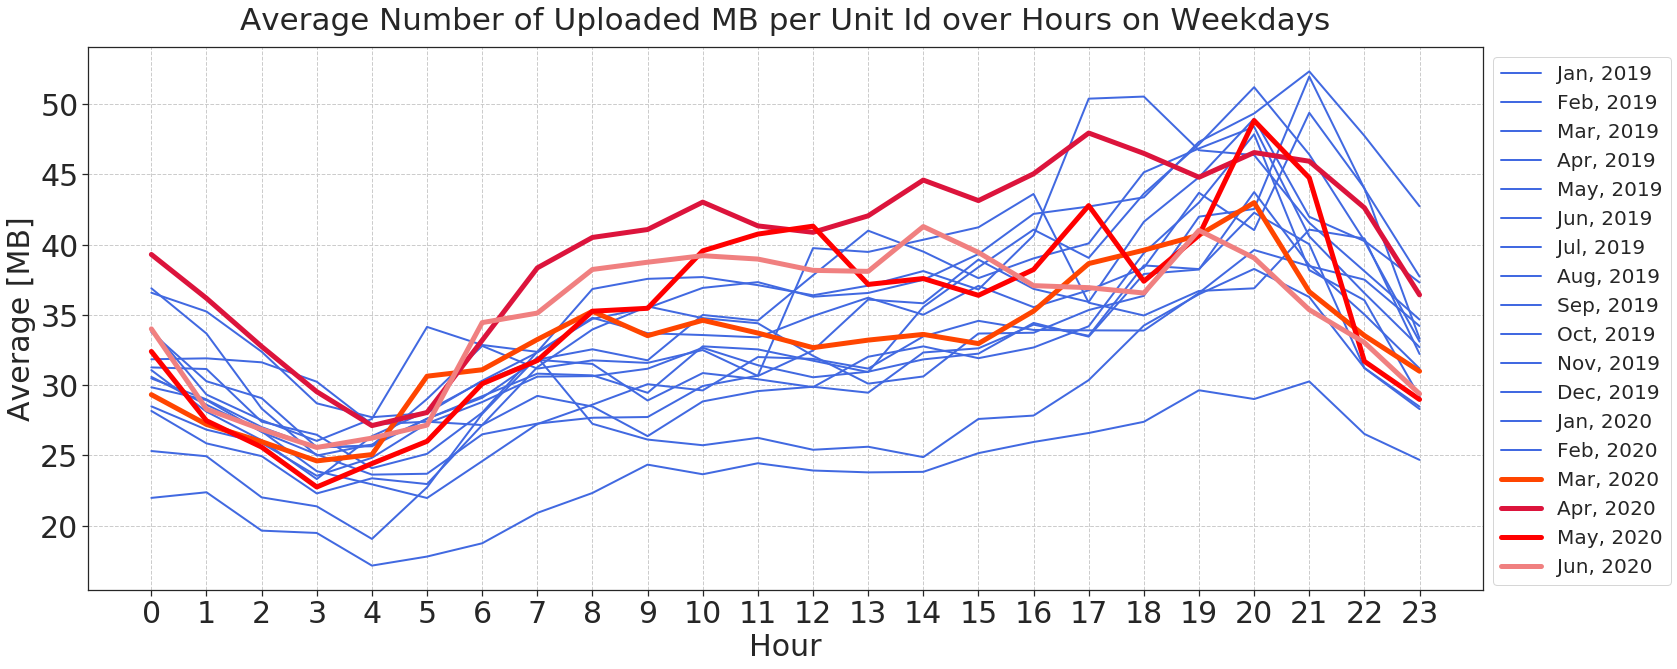
\includegraphics[width=.49\textwidth]{figs/wenjun/upload_wdays_compare.png}
  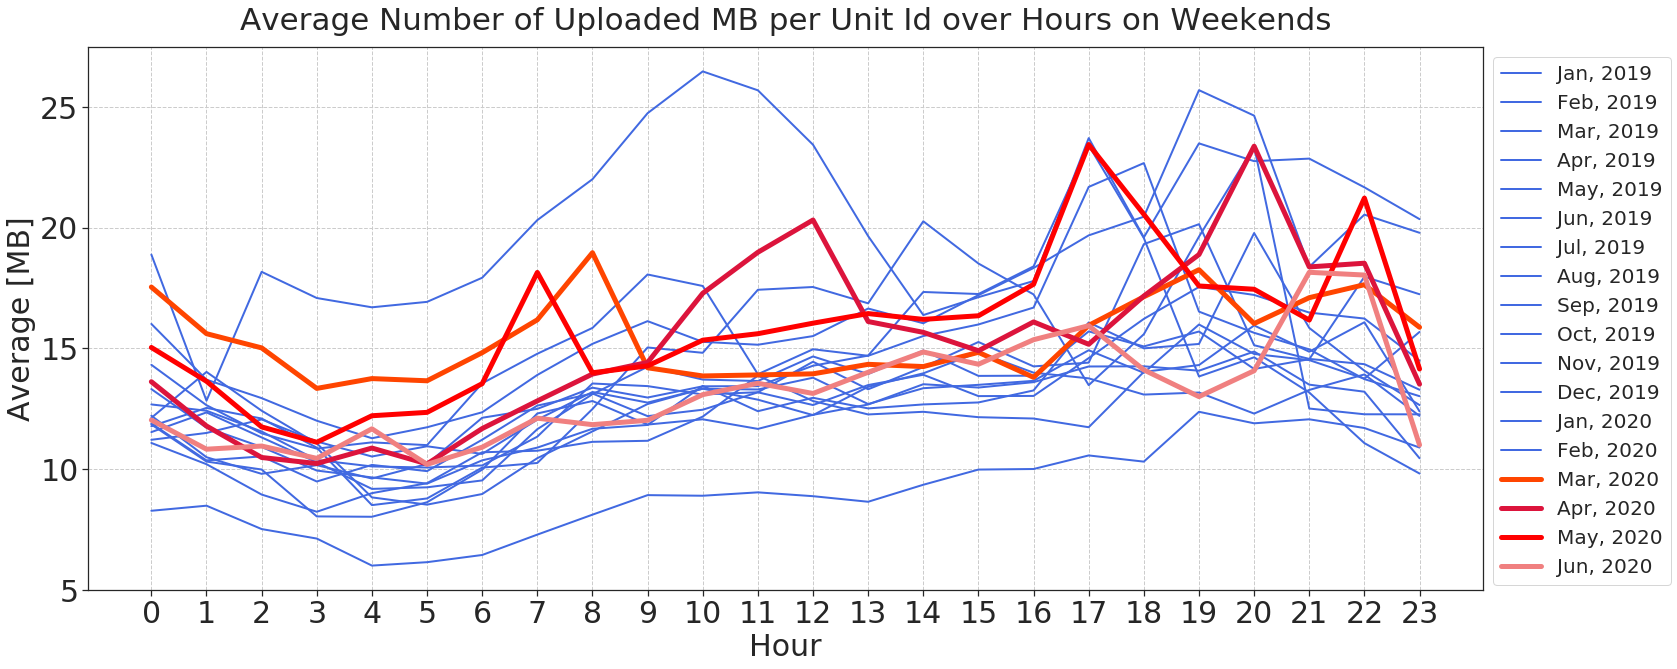
\includegraphics[width=0.49\textwidth]{figs/wenjun/upload_wends_compare.png}

  \vspace*{-1em}
  \caption{TODO: Upload Data.}
    \vspace*{-1em}
  \label{fig:upload_data_per_user_hours_fig}  
\end{figure*}

\subsubsection{Average Upload Data per User}
\label{sec:upload-data-per-user-over-hours}

The upload data is the number of bytes that the customer transmitted from wired LAN devices and Wi-Fi devices to the internet. As shown in the Figure \ref{fig:upload_data_per_user_hours_fig}, compare with the pattern in average download data, the lines in the upload data graph is more fluctuating, especially the pattern for the upload data on weekends. 

\textbf{TODO: need more analysis (not sure yet); updating the comparison graph}


% (This part may not be important, can't show the difference between after covid-19 and before covid-19)
% \subsubsection{Average Download Data v.s. Average Upload Data}
% \label{sec:download_upload_comparison}

% We compare the average number of download data and that of upload data per user over hours after COVID-19 on both weekdays and weekends. As shown in Figure \ref{fig:download_upload_compare}, we can see that the average number of download data is much larger than that of upload data. 

% % Comparison
% \begin{figure*}[t]
%   \centering
%   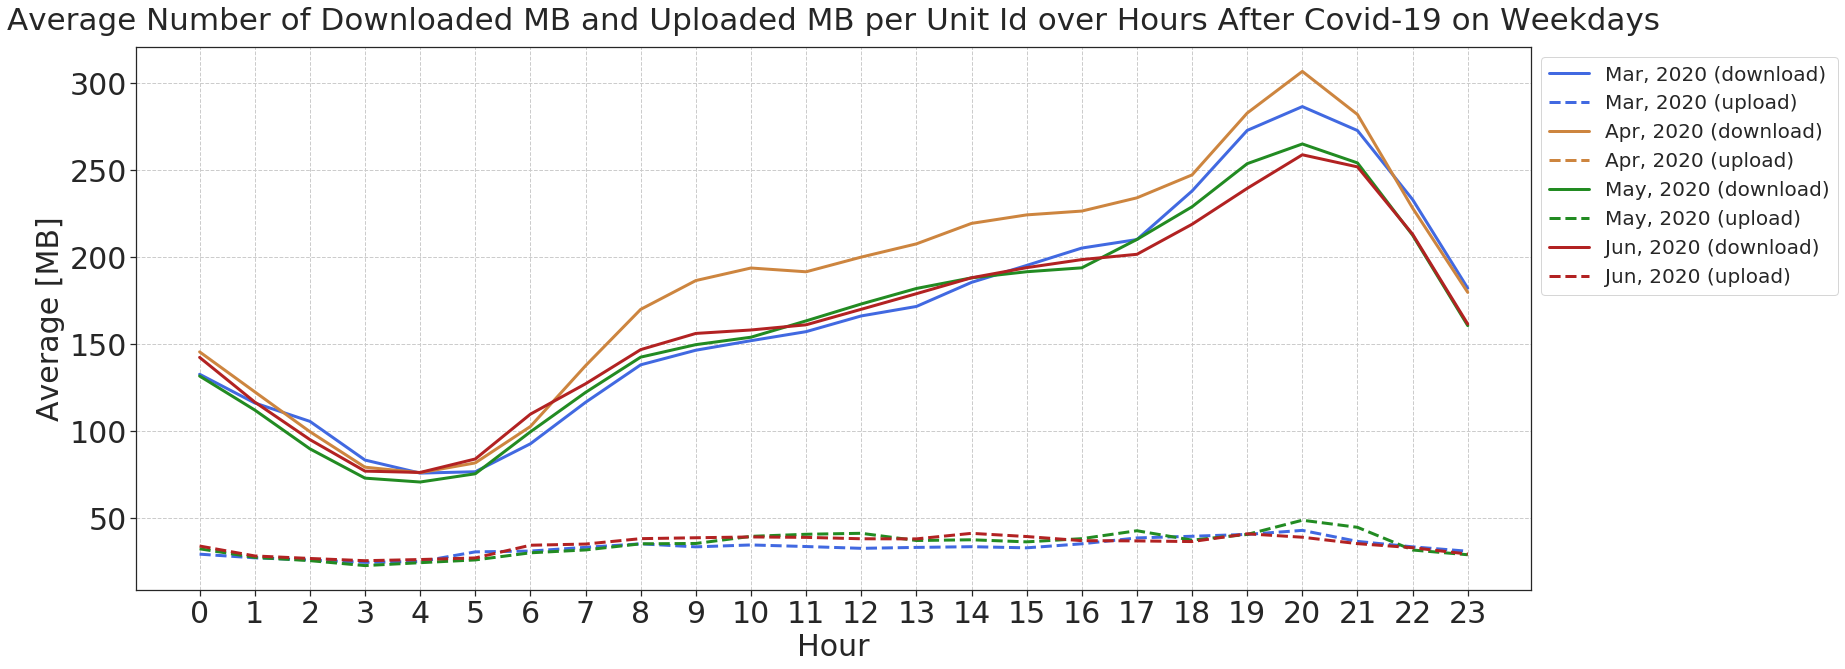
\includegraphics[width=.49\textwidth]{figs/wenjun/weekdays_comparison.png}
%   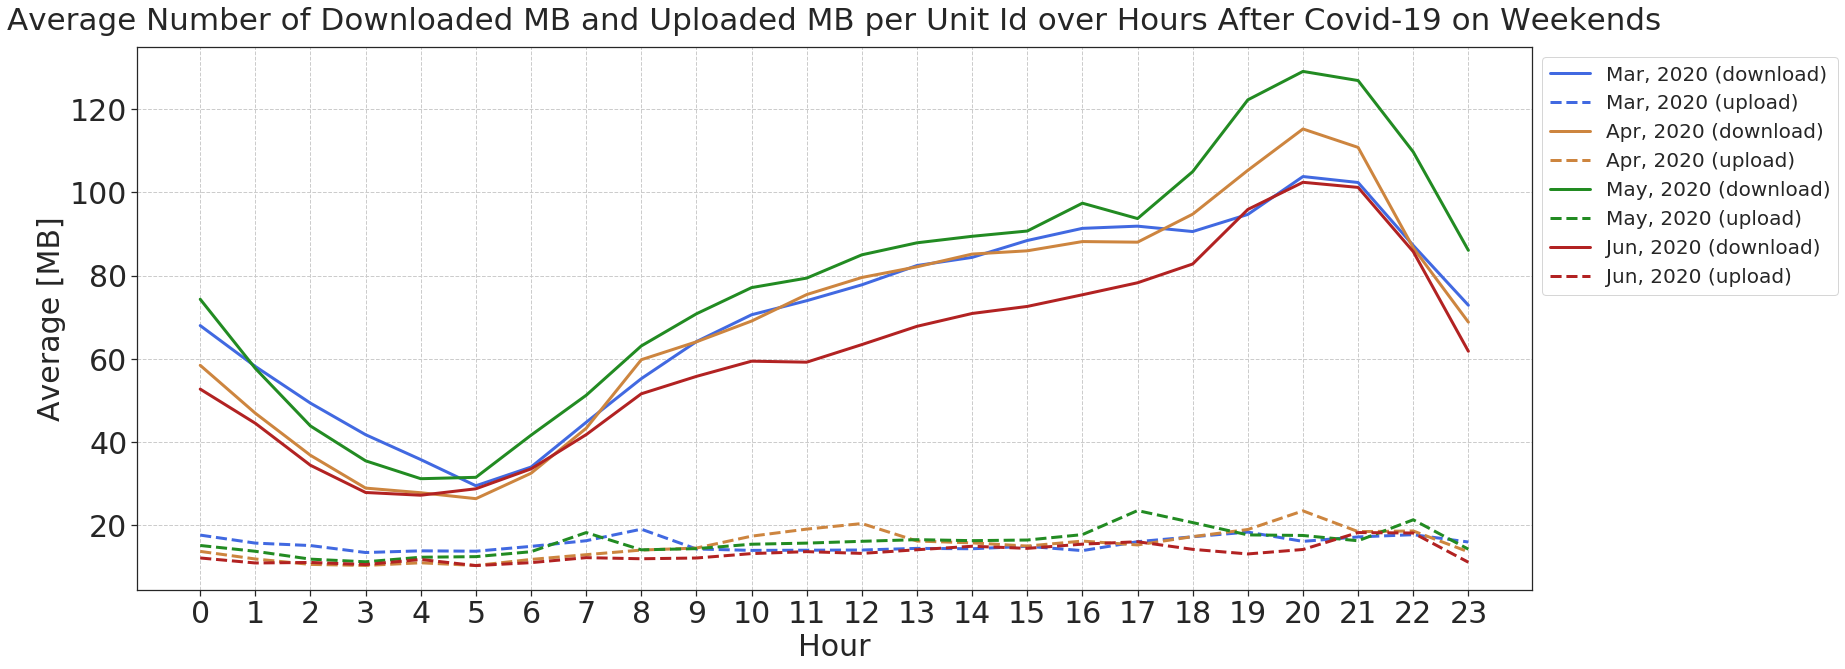
\includegraphics[width=.49\textwidth]{figs/wenjun/weekends_comparison.png}

%   \vspace*{-1em}
%   \caption{caption: Comparison.}
%     \vspace*{-1em}
%   \label{fig:download_upload_compare}  
% \end{figure*}

\section{Challenges}
\label{sec:challenges}
Because we was working with a big data set, in total \SI{300}{\giga\byte} of data, one of the main challenges that we faced was to find an application that would be able to process all this data. By talking to my supervisors, we decided to use a virtual machine on Google Cloud because we thought it would be enough to treat and process all the data sets. However, even using Google Cloud, the virtual machine run out of memory and it was necessary find different ways to storage the data, such as transitioning to BigQuery. Moreover, even though this is a professional data set gathered by FCC, there was still some invalided and noisy data and some lack of data description, e.g., outdated information about Whiteboxes. These implications related to the data set also led to some additional challenges to analyze it.

\section{Conclusion}
\label{sec:conclusion}

Based on the graphs and information presented, it is possible to conclude that the COVID-19 outbreak has impacted the consume of Internet in the US. In terms of average consumption per user, from January 2020 to March 2020 (before and after COVID-19 hit the country) increased by \SI{53}{\percent} for downloaded data and by \SI{38}{\percent} for uploaded data. In addition to that, approximately \SI{70}{\percent} of consumers experienced a decrease in their average download speed in March if compared to their average download speed in January, and approximately \SI{80}{\percent} of users noticed a decrease in their average upload speed. These numbers show some of the impacts of COVID-19 in  Internet usage since this has been the most influential external factor to  Internet consumption in the US. Through these results that show that people indeed consumed more data in March, it can be inferred that people tended to comply to the stay at home orders and started doing most of their daily activities e.g., work and study, in a virtual environment.

\subsection{Future Work}
\label{sec:future-work}

As this project is a working in progress, some of the next steps would be continuing analyzing the changes in  Internet consumption, e.g., how consumption changed in business hours and changes related to different geographic regions in the US, and also analyzing changes in latency.

\section{Acknowledgements}
\label{sec:acknowledgements}

We would like to thank Barnard Computer Science department and the DIMACS REU program for making this summer research project possible to be accomplished and also the Craig Newmark Philanthropies for funding this research project.

\bibliographystyle{IEEEtran}
\bibliography{bibs/references}
\end{document}
